\section{Kollision von Dense Units}

Da die Dense Units auch in unterschiedlichen Dimensionen existieren können, müssen diese als solche gekennzeichnet werden. In diesem Schritt ist das Subspace Clustering erkennbar. Direkt nach Berechnung der Dense Units, werden diese mit anderen Dense Units verglichen, um höhere Subspaces zu finden. Um Kollisionen in den Dense Units festzustellen, muss jedem Punkt im Datenset eine hohen Zufallszahl zugewiesen werden. Dieser Schritt wird vor dem Ausführen des SUBSCALE Algorithmus durchgeführt. Für alle Dense Units werden Signaturen gebildet. Diese Signatur ist die Summe aller Punkte in der Dense Unit. Anhand dieser Signatur werden die Dense Units in eine Tabelle eingetragen, mit den dazugehörigen Punkten und der Dimension. Bei einer Kollision der Signaturen, wird die Dimension zu dem bereits vorhanden Eintrag hinzugefügt (siehe Abbildung \ref{dense-collision}). \cite{Ramin}

\begin{figure}[h]
	\centering
	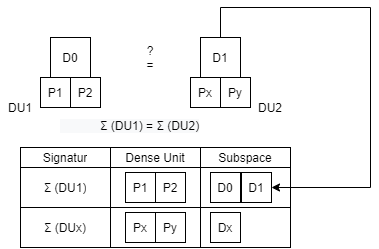
\includegraphics[width=0.5\textwidth]{DenseUnitKollision.png}
	\caption{Kollisionsauflösung von Dense Units}
	\label{dense-collision}
\end{figure}


